\documentclass[10pt,c,aspectratio=1610,handout]{beamer}
\usetheme[block=fill,numbering=fraction,progressbar=frametitle]{metropolis}
%\usecolortheme{beaver}
\usepackage{textpos}
\usepackage{amsmath}
\usepackage{amssymb}
\usepackage{appendixnumberbeamer}

\setbeamercovered{transparent}

\newcommand\blfootnote[1]{%
  \begingroup
  \renewcommand\thefootnote{}\footnote{#1}%
  \addtocounter{footnote}{-1}%
  \endgroup
}

\newtheorem{claim}{Claim}
\newtheorem{conjecture}{Conjecture}
\newtheorem{remark}{Remark}

\renewcommand{\baselinestretch}{1.25}
% Colour theme
\definecolor{QDMblue}{rgb}{0.00, 0.1882, 0.3608}
\definecolor{QDMgold}{rgb}{0.9098, 0.6510, 0.0000}
\definecolor{QDMgreen}{rgb}{0.3098, 0.5490, 0.0510}
\setbeamercolor{normal text}{ fg= QDMblue , bg= white }
\setbeamercolor{alerted text}{ fg= QDMgold }
\setbeamercolor{example text}{ fg= QDMgreen }

\begin{document}

% Personal Info
\title{Lecture 05: Capital Stocks and Taxes}
\author[Konstantin Gantert]{\begin{large} Konstantin Gantert \end{large} \\ \textbf{Quantitative Dynamic Macroeconomics}}
\date{\textit{this version:} \today}

% Eliminates Navigation Bar on every Frame
\beamertemplatenavigationsymbolsempty

%-------------------------------------------------------------------------
% 0.1 Titlepage
%-------------------------------------------------------------------------
{\setbeamertemplate{footline}{} 
\frame{\titlepage}}
 \addtocounter{framenumber}{-1}
%-------------------------------------------------------------------------
% ABOUT THE LECTURE
%-------------------------------------------------------------------------
% Outline for this Lecture
\begin{frame}{Outline for this Lecture}%
  \onslide<1->{%
  \begin{minipage}{0.48\textwidth}%
    \textbf{What have we seen so far}%
    \begin{enumerate}%
      \item Monetary policy rules {\tiny [CG 6]}%
      \item Monopolistic competition {\tiny [CG 1, 3, 5]}%
      \item Information frictions {\tiny [CG 1, 5]}%
      \item Impulse response functions {\tiny [CG 3, 4]}%
    \end{enumerate}%
  \end{minipage}}%
  \hfill%
  \onslide<3->{%
  \begin{minipage}{0.48\textwidth}%
    \textbf{What we will see today}%
    \begin{enumerate}%
      \item A model of money and capital {\tiny [CG 1, 5]}%
      \item Equilibrium tax distortions {\tiny [CG 5, 6]}
      \item Optimal labor \& capital taxation  {\tiny [CG 3, 6]}%
    \end{enumerate}%
  \end{minipage}}%
  \vspace*{0.25in}%
  \onslide<2->{%
  \begin{block}{Big Picture of the Lecture:}%
    \begin{enumerate}%
      \item How does capital change the behavior of our model economy?%
      \item How do taxes and government spending impact our model economy?%
      \item Can we derive some policy prescriptions from the model?%
    \end{enumerate}%
  \end{block}}%
\end{frame}%
%-------------------------------------------------------------------------
% BLOCK 1: A Model of Money and Capital
%-------------------------------------------------------------------------
\section{A Model of Money and Capital\\{\small Model Setup - Cole (2020) chapter 14}}%
%-------------------------------------------------------------------------
% A Capital Stock Law of Motion
\begin{frame}{A Capital Stock Law of Motion}%
  \begin{itemize}%
    \item[$\blacktriangleright$] We will assume that the final good (output) can now be used ...%
    \begin{itemize}%
      \item[$\rightarrow$] either in the form of consumption $C_{t}$,%
      \item[$\rightarrow$] or in the form of investment $X_{t}$.%
    \end{itemize}%
    \vspace*{0.2in}%
    \pause%
    \item[$\blacktriangleright$] Denote household beginning-of-period capital stock as $K_{t}$.%
    \begin{itemize}%
      \item[$\rightarrow$] So that the date $t$ state has date $t$ variables.%
    \end{itemize}%
    \vspace*{0.2in}%
    \pause%
    \item[$\blacktriangleright$] The equation of motion for the capital stock is:%
    \begin{align*}%
      K_{t+1} \; = \; (1-\delta )K_{t}+X_{t}%
    \end{align*}%
  \end{itemize}%
\end{frame}%
%-------------------------------------------------------------------------
% Production and Resources in the Capital Stock Model
\begin{frame}{Production and Resources in the Capital Stock Model}%
  \begin{itemize}%
    \item[$\blacktriangleright$] Households produce the final good according to a Cobb-Douglas production function:%
    \begin{itemize}%
      \item[$\rightarrow$] Both labor and capital are essential input factors of production.%
      \item[$\rightarrow$] Production is subject to a labor-augmenting productivity growth factor $Z_{t}$.%
    \end{itemize}%
    \vspace*{0.2in}%
    \pause%
    \item[$\blacktriangleright$] The resource constraint for the economy is now given by:%
    \begin{align*}%
      \left[ Z_{t}L_{t}\right]^{1-\alpha }K_{t}^{\alpha } \; = \; C_{t} + X_{t}%
    \end{align*}%
    \pause%
    \item[$\blacktriangleright$] Labor augmenting technical change is a necessary assumption for a balanced growth path:%
    \begin{itemize}%
      \item[$\rightarrow$] It is equivalent to total factor productivitz, $Z_t^{1-\alpha} \; = \; \tilde Z_t$.%
      \item[$\rightarrow$] Along balanced growth path (BGP), capital will grow at same rate as $Z_t$ not $\tilde Z_t$.
      \item[$\rightarrow$] It follows, that output is growing at the same rate.%
    \end{itemize}%
  \end{itemize}%
\end{frame}%
%-------------------------------------------------------------------------
% Marginal Productivities of Labor and Capital (1/2)
\begin{frame}{Marginal Productivities of Labor and Capital (1/2)}%
  The \textbf{Cobb-Douglas production function}, $\left[ Z_{t}L_{t}\right]^{1-\alpha}K_{t}^{\alpha}$, has many nice features:%
  \vspace*{0.15in}%
  \begin{itemize}%
    \item[$\blacktriangleright$] If labor and capital double, so does output: \emph{constant returns to scale}.%
    \pause%
    \item[$\blacktriangleright$] The marginal products of labor and capital are given by:%
    \begin{align*}
      MPL \; = & \; (1-\alpha )Z_{t}^{1-\alpha }L_{t}^{-\alpha }K_{t}^{\alpha }\\%
      MPK \; = & \; \alpha \left[ Z_{t}L_{t}\right] ^{1-\alpha }K_{t}^{\alpha -1}%
    \end{align*}%
    \vspace*{-0.25in}%
    \pause%
    \begin{itemize}%
      \item[$\rightarrow$] If labor is constant and both capital and productivity grow at the same rate, then the marginal product of capital, is constant.%
      \item[$\rightarrow$] The marginal product of labor grows with productivity.%
      \item[$\rightarrow$] This will turn out to lead to nice long-run growth predictions.%
    \end{itemize}%
  \end{itemize}%
\end{frame}%
%-------------------------------------------------------------------------
% Marginal Productivities of Labor and Capital (2/2)
\begin{frame}{Marginal Productivities of Labor and Capital (2/2)}%
  The \textbf{Cobb-Douglas production function}, $\left[ Z_{t}L_{t}\right]^{1-\alpha}K_{t}^{\alpha }$, has many nice features:%
  \vspace*{0.15in}%
  \begin{itemize}%
    \item[$\blacktriangleright$] The shares paid out to labor and capital are constant over time. They are defined by:%
    \begin{align*}%
      MPL\ast L \; = & \; (1-\alpha )Y_{t}\\%
      MPK\ast K \; = & \; \alpha \ast Y_{t}%
    \end{align*}%
    \vspace*{0.1in}%
    \pause%
    \item[$\blacktriangleright$] How do capital and labor inputs respond to price changes? In an optimal program, it follows that:%
    \begin{align*}%
      \frac{MPL}{MPK} \; = & \; \frac{w}{r} \; = \; \frac{(1-\alpha )K}{\alpha L}\\%
      \implies \quad d log \left(\frac{w}{r} \right) \; = & \; d log \left( \frac{K}{L} \right)%
    \end{align*}%
    \textbf{Interpretation:} A 1 percent change in the ratio of input prices changes the relative inputs by 1 percent: unit elasticity (special feature of Cobb-Douglas functions).%
  \end{itemize}%
\end{frame}%
%-------------------------------------------------------------------------
% Aggregation of a Representative Agent Economy
\begin{frame}{Aggregation of a Representative Agent Economy}%
  \begin{block}{Approach}%
    Because we have a representative agent economy again (since there is only a single good and all households end up being the same), we will not distinguish between a household's choice of labor, investment, and capital, and the aggregate choices.%
  \end{block}%
  \vspace*{0.2in}%
  \pause%
  This is a serious abuse of notation and we need to be careful not to confuse ourselves:%
  \begin{itemize}%
    \item[$\blacktriangleright$] The transition equation for capital holds at the level of the household.%
    \item[$\blacktriangleright$] However, the resource constraint holds at the level of the economy.%
    \pause%
    \item[$\blacktriangleright$] A household simply takes prices as given and chooses its optimal plan.%
    \item[$\blacktriangleright$] However, prices are endogenous at the level of the economy.%
  \end{itemize}%
\end{frame}%
%-------------------------------------------------------------------------
% Household Optimization Problem with Capital
\begin{frame}{Household Optimization Problem with Capital}
  Assume \emph{perfect foresight}, so the \textbf{households's problem} is choosing a sequence to maximize%
  \begin{align*}%
    \max_{\left\{ C_{t},L_{t},M_{t+1},B_{t+1},K_{t+1}\right\}_{t=1}^{2}} \sum_{t=1,2} \beta^{t-1} \left[ u(C_{t})-v(L_{t}) \right] + \beta^{2}V(M_{3},B_{3},K_{3})%
  \end{align*}%
  subject to%
  \begin{align*}%
    M_{t} \; \geq \; P_{t} C_{t}%
  \end{align*}%
  and%
  \begin{align*}%
    & \; P_{t} \left[ \left[ Z_{t} L_{t}\right]^{1-\alpha} K_{t}^{\alpha} - \delta K_{t} \right] +\left[ M_{t}-P_{t}C_{t} \right] + B_{t} + T_{t} \\%
    \geq & \; M_{t+1} + q_{t} B_{t+1} + P_{t} \left[ K_{t+1}-K_{t} \right] \quad \forall t \leq 2.%
  \end{align*}%
  \vspace*{-0.2in}%
  \pause%
  \begin{itemize}%
    \begin{small}%
      \item[$\blacktriangleright$] Only consumption shows up in the HH's CiA constraint because new investment is transacted in the asset market or HH has more efficient means of making large purchases such as capital.%
      \pause%
      \item[$\blacktriangleright$] Budget constraint deals with capital depreciation by subtracting the depreciated component from output so HH picks the new capital stock: choice variable is $K_{t+1}$.%
    \end{small}%
  \end{itemize}%
\end{frame}%
%-------------------------------------------------------------------------
% Household FOCs with Capital (1/2)
\begin{frame}{Household FOCs with Capital (1/2)}%
  \begin{itemize}%
    \item[$\blacktriangleright$] The \textbf{consumption FOC} is \emph{unchanged}:%
    \begin{align*}%
      \beta^{t-1}u^{\prime}(C_{t}) -P_{t} \left[ \lambda_{t}+\mu_{t}\right] \; = \; 0%
    \end{align*}%
    \vspace*{0.15in}%
    \pause%
    \item[$\blacktriangleright$] The \textbf{labor FOC} has \emph{changed} (similar to before except that the MPL now shows $L$ and $K$):%
    \begin{align*}%
      -\beta^{t-1} v^{\prime}(L_{t}) + \mu _{t} P_{t} \underbrace{Z_{t}^{1-\alpha} (1-\alpha) L_{t}^{-\alpha} K_{t}^{\alpha}}_{MPL} \; = \; 0%
    \end{align*}%
    \vspace*{0.15in}%
    \pause%
    \item[$\blacktriangleright$] The \textbf{money and bond FOCs} are also \emph{unchanged} and are given by:%
    \begin{align*}%
      -\mu_{t} + \lambda_{t+1} + \mu_{t+1} \; = & \; 0\\%
      -\mu_{t} q_{t} + \mu_{t+1} \; = & \; 0%
    \end{align*}%
  \end{itemize}%
\end{frame}%
%-------------------------------------------------------------------------
% Household FOCs with Capital (2/2)
\begin{frame}{Household FOCs with Capital (2/2)}%
  \begin{itemize}%
    \item[$\blacktriangleright$] The new condition coming for \textbf{choice of capital stock} at the end of period:%
    \begin{align*}%
      -\mu _{t} P_{t} + \mu_{t+1} P_{t+1} \left[ \left[ Z_{t+1} L_{t+1} \right]^{1-\alpha} \alpha K_{t+1}^{\alpha-1} + 1 - \delta \right] \; = \; 0%
    \end{align*}%
    \pause%
    \begin{itemize}%
      \item[$\rightarrow$] The capital FOC is similar to the bond FOC, as it connects today's and tomorrow's budget constraint.%
      \item[$\rightarrow$] The main difference is that the payoff of capital is defined by the $MPK$ instead of a nominal market interest rate, $\frac{1}{q}$.%
    \end{itemize}%
    \vspace*{0.15in}%
    \pause%
    \item[$\blacktriangleright$] In total, these FOCs along with the CiA constraint, the budget constraint, the resource constraint and the market clearing conditions for money and bonds give \textbf{the constraints that our equilibrium must satisfy!}%
  \end{itemize}%
\end{frame}%
%-------------------------------------------------------------------------
% BLOCK X: Accounting for Growth
%-------------------------------------------------------------------------
\section{Accounting for Growth\\{\small Cole (2020) chapter 14}}%
%-------------------------------------------------------------------------
% Growth Accounting for Productivity and Money
\begin{frame}{Growth Accounting for Productivity and Money}%
  \begin{itemize}%
    \item[$\blacktriangleright$] The presence of money growth and productivity growth means that our economy is not going to be stationary.%
    \pause%
    \item[$\blacktriangleright$] Assume that both productivity and the money supply grow at constant rates and normalize initial values to get%
    \begin{align*}%
      Z_{t} \; = \; (1+g)^{t-1} Z_1 \; = \; (1+g)^{t-1},%
    \end{align*}%
    and%
    \begin{align*}%
      M_{t} \; = \; (1+\tau )^{t-1} M_1 \; = \; (1+\tau )^{t-1}%
    \end{align*}%
  \end{itemize}%
\end{frame}%
%-------------------------------------------------------------------------
% Output and Capital Growth
\begin{frame}{Output and Capital Growth}%
  \vspace{0.2in}%
  \begin{block}{Solution Approach}%
    In order to derive a \textbf{perfect foresight solution} of the model, we apply the following steps:\\%
    \vspace{-0.025in}%
    \begin{itemize}%
      \item[$\blacktriangleright$] Conjecture that capital grows at the same rate as productivity!
      \item[$\blacktriangleright$] Conjecture that labor is constant!%
      \item[$\blacktriangleright$] Conjecture that the \emph{cash-in-advance constraint holds as an equality}.%
    \end{itemize}%
    \vspace{-0.05in}%
    \pause%
    It follows, that we can derive a solution to the model that only depends on the initial allocation and the \emph{constant} growth rates!%
  \end{block}%
  \pause%
  \begin{itemize}%
    \item[$\blacktriangleright$] This implies that output will grow at rate $g$ since%
    \begin{align*}%
      Y_{t} \; = & \; \left[ Z_{t} L \right]^{1-\alpha} K_{t}^{\alpha} \; = \; Z_t L \left[\frac{Z_t L}{K_t}\right]^{-\alpha}\\%
      Y_{t-1} \; = & \; \left[ Z_{t-1} L \right]^{1-\alpha} K_{t-1}^{\alpha} \; = \; Z_{t-1} L \left[\frac{Z_{t-1} L}{K_{t-1}}\right]^{-\alpha}\\%
      \implies Y_{t} \; = & \; (1+g) Y_{t-1} \; = \; Z_{t} Y_{1} \quad \text{given } Z_1=1%
    \end{align*}%
  \end{itemize}%
  \vspace*{0.15in}%
\end{frame}%
%-------------------------------------------------------------------------
% Consumption Growth
\begin{frame}{Consumption Growth}%
  \begin{small}%
    \begin{block}{\small Conjectured capital growth rate}%
      Since capital is assumed to grow at the same rate as productivity%
      \begin{align*}%
        K_{t} \; = \; (1+g) K_{t-1} \; = \; Z_{t} K_{1},%
      \end{align*}%
      it follows that the capital stock is defined by initial capital and productivity growth.%
    \end{block}%
  \end{small}%
  \pause%
  The conjecture further implies:%
  \begin{itemize}%
    \item[$\blacktriangleright$] \textbf{Investment} also grows at a constant rate defined by:%
    \begin{align*}%
      X_{t} \; = \; (1+g) K_{t} - (1-\delta) K_{t} \; = \; (g + \delta) Z_{t} K_{1}%
    \end{align*}%
    \vspace*{-0.2in}%
    \pause%
    \item[$\blacktriangleright$] Substituting for both the production function and investment in the \textbf{resource constraint}:%
    \begin{align*}%
      \left[ Z_{t} L \right]^{1-\alpha} K_{t}^{\alpha} \; = & \; C_{t} + \left[ g+\delta \right] K_{t} \\%
      \implies \quad Z_{t} L^{1-\alpha} K_{1}^{\alpha} \; = & \; C_{t} + \left[ g+\delta \right] Z_{t} K_{1}%
    \end{align*}%
    \vspace*{-0.2in}%
    \pause%
    \item[$\blacktriangleright$] As everything else except labor grows at rate $g$, so \textbf{consumption} must grow at $g$ as well:%
    \begin{align*}%
      C_1 \; = & \; L^{1-\alpha} K_{1}^{\alpha} - \left[ g+\delta \right] K_{1}%
    \end{align*}%
  \end{itemize}%
\end{frame}%
%-------------------------------------------------------------------------
% Price Level Growth
\begin{frame}{Price Level Growth}%
  \begin{itemize}%
    \item[$\blacktriangleright$] Assume that the \textbf{cash-in-advance} constraint always holds with equality. It follows:%
    \begin{align*}%
      P_{t} \; = \; \frac{M_{t}}{C_{t}}=\frac{(1+\tau )}{(1+g)}P_{t-1}%
    \end{align*}%
    \item[$\blacktriangleright$] \emph{Essentially the same result} derived previously when output was only produced with labor.%
  \end{itemize}%
\end{frame}%
%-------------------------------------------------------------------------
% BLOCK X: Rendering the Model Stationary
%-------------------------------------------------------------------------
\section{Rendering the Model Stationary\\{\small Cole (2020) chapter 14}}%
%-------------------------------------------------------------------------
% Change-in-Variables: Consumption
\begin{frame}{Change-in-Variables: Consumption}%
  Let's rewrite our model in \textbf{stationary terms} again using a change-in-variables transformation!%
  \pause%
  \begin{itemize}%
    \item[$\blacktriangleright$] Assuming \emph{log utility}, our \textbf{consumption FOC} is:%
    \begin{align*}
      \beta^{t-1} \frac{1}{C_{t}} \; = & \; \left[ \lambda_{t}+\mu_{t} \right] P_{t} \; = \; \left[ \lambda_{t}+\mu_{t} \right] \frac{M_{t}}{C_{t}} \\%
      \implies \beta^{t-1} \; = & \; \left[ \lambda_{t}+\mu_{t}\right] (1+\tau)^{t-1} M_{1}%
    \end{align*}%
    \pause%
    \item[$\blacktriangleright$] Once again, we make a \textbf{change in variables}, setting:%
    \begin{align*}%
      \tilde{\lambda}_{t} \; = & \; \lambda_{t} \frac{(1+\tau)^{t-1}}{\beta^{t-1}}\\%
      \tilde{\mu}_{t} \; = & \; \mu_{t} \frac{(1+\tau)^{t-1}}{\beta^{t-1}}%
    \end{align*}%
    \pause%
    \item[$\blacktriangleright$] Applying the \emph{change-in-variables} transformation to the \textbf{consumption FOC} gives us:%
    \begin{align*}%
      1 \; = \; \left[ \tilde{\lambda}_{t}+\tilde{\mu}_{t} \right] M_{1} \; = \; \left[ \tilde{\lambda}_{t}+\tilde{\mu}_{t}\right]%
    \end{align*}%
  \end{itemize}%
\end{frame}%
%-------------------------------------------------------------------------
% Change-in-Variables: Labor
\begin{frame}{Change-in-Variables: Labor}%
  \begin{itemize}%
    \item[$\blacktriangleright$] Using the \emph{change-in-variables}, the \textbf{labor FOC} can be rewritten as:%
    \begin{align*}%
      \beta^{t-1} L_{t}^{\gamma} \; = & \; \mu_{t} P_{t} Z_{t}^{1-\alpha} (1-\alpha) L_{t}^{-\alpha} K_{t}^{\alpha}%
    \end{align*}%
    \vspace*{-0.1in}%
    \pause%
    \item[$\blacktriangleright$] Substituting for $P_t$ and simplifying (assuming $Z_1=1$), this leads to:%
    \begin{align*}%
      \beta^{t-1} L_{t}^{\gamma} \; = & \; \mu_{t} \frac{(1+\tau)^{t-1}}{(1+g)^{t-1}} P_{1} Z_{t}^{1-\alpha} (1-\alpha) L_{t}^{-\alpha} K_{t}^{\alpha}\\%
      \Leftrightarrow \quad \beta^{t-1} L^{\gamma +\alpha} \; = & \; \mu_{t} \frac{(1+\tau)^{t-1}}{(1+g)^{t-1}} P_{1} Z_{1}^{1-\alpha} (1-\alpha) K_{1}^{\alpha} (1+g)^{t-1}\\%
      \Leftrightarrow \quad L^{\gamma+\alpha} \; = & \; \tilde{\mu}_{t} P_{1} (1-\alpha) K_{1}^{\alpha}%
    \end{align*}%
    \vspace*{-0.1in}%
    \pause%
    \item[$\blacktriangleright$] The result is close to what we had before, but now also taking the impact of the capital stock on labor into account.%
  \end{itemize}%
\end{frame}%
%-------------------------------------------------------------------------
% Change-in-Variables: Money and Bonds
\begin{frame}{Change-in-Variables: Money and Bonds}%
  \begin{itemize}%
    \item[$\blacktriangleright$] The \textbf{FOCs for money and bonds} can be written as:%
    \begin{align*}%
      \tilde{\mu}_{t} \; = & \; \frac{\beta}{1+\tau} \left[ \tilde{\lambda}_{t+1} + \tilde{\mu}_{t+1} \right] \; = \; \frac{\beta}{1+\tau}\\%
      \tilde{\mu}_{t} q_{t} \; = & \; \frac{\beta}{1+\tau} \tilde{\mu}_{t+1} \implies q_{t} \; = \; \frac{\beta}{1+\tau}%
    \end{align*}%
    \item[$\blacktriangleright$] These are exactly our results from the model with only labor!%
  \end{itemize}%
\end{frame}%
%-------------------------------------------------------------------------
% Change-in-Variables: Capital Stock
\begin{frame}{Change-in-Variables: Capital Stock}%
  \begin{itemize}%
    \item[$\blacktriangleright$] The \textbf{capital FOC} is given by:%
    \begin{align*}%
      \mu _{t} P_{t} \; = \; \mu _{t+1} P_{t+1} \left( \left[ Z_{t+1}L_{t+1} \right]^{1-\alpha} \alpha K_{t+1}^{\alpha-1} + 1 - \delta \right)%
    \end{align*}%
    \pause%
    \item[$\blacktriangleright$] It can be rewritten as follows once we \emph{substitute out for prices}:%
    \begin{align*}%
      \mu_{t} \; = \; \mu_{t+1} \frac{1+\tau}{1+g} \left\{ \alpha \left[ \frac{Z_{t+1}L_{t+1}}{K_{t+1}} \right]^{1-\alpha} + 1 - \delta \right\}%
    \end{align*}%
    \pause%
    \item[$\blacktriangleright$] Since $Z_{t}$ and $K_{t}$ \emph{grow at the same rate} and labor is constant:%
    \begin{align*}%
      \mu_{t} \; = \; \mu_{t+1} \frac{1+\tau}{1+g} \left\{ \alpha \left[ \frac{Z_{1}L}{K_{1}} \right]^{1-\alpha} + 1 - \delta \right\}%
    \end{align*}%
    \pause%
    \item[$\blacktriangleright$] Finally we put in our \emph{change in variables} to get that and $\tilde \mu_t = \tilde \mu_{t+1}$:%
    \begin{align*}%
      1 \; = \; \beta \frac{1}{1+g} \left\{ \alpha \left[ \frac{Z_{1}L}{K_{1}} \right]^{1-\alpha} + 1 - \delta \right\}%
    \end{align*}%
  \end{itemize}%
\end{frame}%
%-------------------------------------------------------------------------
% A Summary of the Capital Stock Model
\begin{frame}{A Summary of the Capital Stock Model}%
  \begin{align}%
    \text{Opt. consumption condition:} & \quad 1 \; = \; \left[ \tilde{\lambda} + \tilde{\mu} \right]\\%
    \text{Opt. labor condition:} & \quad L^{\gamma +\alpha} \; = \; \frac{\beta}{1+\tau} P_{1} (1-\alpha) Z_{1}^{1-\alpha} K_{1}^{\alpha} \label{BG labor}\\%
    \text{Opt. money condition:} & \quad \frac{\beta}{1+\tau} \left[ \tilde{\lambda}+\tilde{\mu} \right] \; = \; \frac{\beta}{1+\tau} \; = \; \tilde{\mu}\\%
    \text{Opt. bond condition:} & \quad q \; = \; \frac{\beta}{1+\tau}\\%
    \text{Opt. capital condition:} & \quad 1 \; = \; \frac{\beta}{1+g} \left\{ \alpha \left[ \frac{Z_{1}L}{K_{1}} \right]^{1-\alpha} + 1 - \delta \right\} \label{BG capital}\\%
    \text{Resource constraint:} & \quad \left[ Z_{1} L \right]^{1-\alpha} K_{1}^{\alpha} \; = \; C_{1} + \left[ g+\delta \right] K_{1}\\%
    \text{CiA constraint:} & \quad P_{1} \; = \; \frac{M_{1}}{C_{1}} \; = \; \frac{1}{C_1}%
  \end{align}%
\end{frame}
%-------------------------------------------------------------------------
% BLOCK XX: Solving for the Balanced-Growth-Path
%-------------------------------------------------------------------------
\section{Solving for the Balanced-Growth-Path\\{\small Cole (2020) chapter 14}}%
%-------------------------------------------------------------------------
% Solving for the BGP of the Capital Stock Model: Approach
\begin{frame}{Solving for the BGP of the Capital Stock Model: Approach}%
  \begin{itemize}%
    \item[$\blacktriangleright$] Our system of equations ...%
    \begin{itemize}%
      \item[$\rightarrow$] has seven variables to solve for $\left[ C_{1},L,P_{1},\tilde{\mu},\tilde{\lambda},q,K_{1}\right]$,%
      \item[$\rightarrow$] and we take as given $Z_{1}$ and $M_{1}$ along with $g$ and $\tau$.%
    \end{itemize}%
    \vspace*{0.2in}%
    \pause%
    \item[$\blacktriangleright$] The one surprise is that we have to ''solve'' for $K_{1}.$
    \begin{itemize}%
      \item[$\rightarrow$] The initial level of the capital stock must be consistent with balanced growth.%
      \item[$\rightarrow$] Hence, we are assuming to be on the balanced growth path from the beginning.%
    \end{itemize}%
    \vspace*{0.2in}%
    \pause%
    \item[$\blacktriangleright$] Fortunately, our system is again block recursive so we can solve things in steps.%
  \end{itemize}%
\end{frame}%
%-------------------------------------------------------------------------
% Step 1: Solving for the Consumption BGP
\begin{frame}{Step 1: Solving for the Consumption BGP}%
  \begin{itemize}%
    \item[$\blacktriangleright$] Let's start with the \textbf{resource constraint:}%
    \begin{align*}%
      C_{1} \; = \; \left[ Z_{1} L \right]^{1-\alpha} K_{1}^{\alpha} - \left[ g+\delta \right] K_{1}%
    \end{align*}%
    \vspace*{-0.15in}%
    \begin{itemize}%
      \item[$\rightarrow$] Hence, if we know $K_{1}$ and $L$ we know $C_{1}$.%
    \end{itemize}%
    \vspace*{0.3in}%
    \pause%
    \item[$\blacktriangleright$] Move to the \textbf{price condition} and substitute for $C_{1}$:%
    \begin{align*}%
      P_{1} \; = \; \frac{M_{1}}{\left[ Z_{1} L \right]^{1-\alpha} K_{1}^{\alpha} - \left[ g+\delta \right] K_{1}}%
    \end{align*}%
    \vspace*{-0.15in}%
    \begin{itemize}%
      \item[$\rightarrow$] Hence, the initial price level is also determined by $K_{1}$ and $L$.%
    \end{itemize}%
  \end{itemize}%
\end{frame}%
%-------------------------------------------------------------------------
% Step 2: Solving for the Labor-Capital Ratio BGP
\begin{frame}{Step 2: Solving for the Labor-Capital Ratio BGP}%
  \begin{itemize}%
    \item[$\blacktriangleright$] We can solve for $K_{1}$ and $L$ as a simultaneous block given these results.%
    \pause%
    \item[$\blacktriangleright$] Start with our optimality condition for \textbf{capital}. It only depends on $K_{1}$ and $L$:%
    \begin{align*}%
      1 \; = \; \frac{\beta}{1+g} \left\{ \alpha \left[ \frac{Z_{1} L }{K_{1}} \right]^{1-\alpha} + 1 - \delta \right\}.%
    \end{align*}%
    \vspace*{0.1in}%
    \pause%
    \item[$\blacktriangleright$] We solve this equation for the ratio of productive labor, $Z_1 L$, to capital, $K$:%
    \begin{align}%
      \frac{Z_{1} L}{K_{1}} \; = \; \left\{ \frac{1}{\alpha} \left( \frac{1 +g}{\beta} - 1 + \delta \right) \right\}^{1/(1 -\alpha)} \label{PrLtoKratio}%
    \end{align}%
    \vspace*{-0.1in}%
    \begin{itemize}%
      \item[$\rightarrow$] The \textbf{productive-labor-to-capital ratio} depends on the discount rate, the level of productivity growth, and the depreciation rate, but not the rate of inflation.%
      \item[$\rightarrow$] Surprisingly the capital-to-labor ratio is negatively affected by growth.%
    \end{itemize}%
  \end{itemize}%
\end{frame}%
%-------------------------------------------------------------------------
% Step 3: Solving for the Labor BGP
\begin{frame}{Step 3: Solving for the Labor BGP}%
  \begin{itemize}%
    \item[$\blacktriangleright$] To simplify further, \emph{substitute} for $P_{1}$ and for $\tilde{\mu }$ in our \textbf{optimal labor condition:}%
    \begin{align*}
      L^{\gamma+\alpha} \; = \; \left[ \frac{\beta}{1+\tau} \frac{1}{M_{1}} \right] (1-\alpha) Z_{1}^{1-\alpha} K_{1}^{\alpha} \left[ \frac{M_{1}}{\left[ Z_{1} L \right]^{1-\alpha} K_{1}^{\alpha} - \left[ g+\delta \right] K_{1}}\right]%
    \end{align*}%
    \pause%
    \item[$\blacktriangleright$] Multiplying the right-hand-side with $\frac{L^{-1}}{L^{-1}}$, we can derive a \textbf{optimal labor condition} that only depends on the labor-to-capital ratio:%
    \begin{align}%
      L^{1 +\gamma} \; = \; \left[ \frac{\beta}{1+\tau} \right] (1-\alpha) Z_{1}^{1-\alpha} \left[ \frac{K_{1}}{L} \right]^{\alpha} \left[ \frac{1}{\left[ Z_{1} \right]^{1-\alpha} \left[ \frac{K_{1}}{L} \right]^{\alpha} -\left[ g +\delta \right] \frac{K_{1}}{L}} \right] \label{BGFLabor}%
    \end{align}%
    \vspace*{-0.15in}%
    \begin{itemize}%
      \item[$\rightarrow$] Once again we see money growth depressing labor in essentially the exact same way as in our simple model, in which output was produced with labor.%
    \end{itemize}%
    \vspace*{0.15in}%
    \pause%
    \item[$\blacktriangleright$] Once we have solved (\ref{PrLtoKratio}), we can substitute here to get $L$.%
    \item[$\blacktriangleright$] Once we have solved for $L$ and $K_{1},$ we can easily determine the rest of our variables.%
  \end{itemize}%
\end{frame}%
%-------------------------------------------------------------------------
% Kaldor's Long-Run Growth Facts
\begin{frame}{Kaldor's Long-Run Growth Facts}%
  Nicholas Kaldor (1961) proposed six statements of economic growth:%
  \begin{enumerate}%
    \item The growth rate of output per worker is roughly constant over time.%
    \item The growth rate of capital per worker is roughly constant over time {(\scriptsize but varies across countries)}.%
    \item The capital-to-output ratio is roughly constant over time.%
    \item The return on investment is roughly constant over time.%
    \item The real wage grows over time.%
    \item The shares of national income paid to labor and capital are roughly constant over time.%
  \end{enumerate}%
  \vspace*{0.2in}%
  Our model with capital as shown in this lecture is \emph{in line} with those statements!%
\end{frame}%
%-------------------------------------------------------------------------
% BLOCK X: Introducing Labor and Capital Taxes to the Model
%-------------------------------------------------------------------------
\section{Introducing Labor and Capital Taxes to the Model\\{\small Cole (2020) chapter 16}}%
%-------------------------------------------------------------------------
% Adding Taxes to our Capital Stock Model
\begin{frame}{Adding Taxes to our Capital Stock Model}%
  In this section, we \textbf{add labor and capital taxes} to our model with capital.%
  \begin{itemize}%
    \item[$\blacktriangleright$] \textbf{Representative agent model:} Focus on aggregate impact as redistribution cannot be analyzed in this framework.% 
  \end{itemize}%
  \vspace*{0.2in}%
  \pause%
  In order to be able to tax labor and capital, it must be \textbf{traded on markets:}%
  \begin{itemize}%
    \item[$\blacktriangleright$] Need to have each household employ outside labor and rent outside capital.%
    \begin{itemize}
      \item[$\rightarrow$] Assume labor and capital rented in competitive markets with prices $w$ and $r$.%
    \end{itemize}
    \vspace*{0.1in}%
    \pause%
    \item[$\blacktriangleright$] Lump-sum transfers give taxes back.%
    \begin{itemize}%
      \item[$\rightarrow$] But one receives a share of total taxes, \textit{not her contribution to the total}.%
    \end{itemize}%
  \end{itemize}%
\end{frame}%
%-------------------------------------------------------------------------
% Labor and Capital Taxes: Setup
\begin{frame}{Labor and Capital Taxes: Setup}%
  Let $\tau _{l}$ and $\tau _{k}$ denote the \textbf{tax rates on capital and labor:}%
  \begin{itemize}%
    \begin{small}%
      \item[$\blacktriangleright$] After-tax level of labor income: $(1-\tau_L) w_{t} L_{t}$%
      \item[$\blacktriangleright$] Labor tax receipts: $\tau_L w_{t} L_{t}$%
      \item[$\blacktriangleright$] After-tax capital income: $(1-\tau_K)r_{t}K_{t}$%
      \begin{itemize}%
        \item[$\rightarrow$] Capital taxation is normally done net of depreciation, but we are going to ignore that.%
      \end{itemize}%
      \item[$\blacktriangleright$] Capital tax receipts: $\tau _{k}r_{t}K_{t}$%
    \end{small}%
  \end{itemize}%
  \pause%
  \vspace*{0.2in}%
  The \textbf{government's per capita transfers} its receipts back to the public:%
  \begin{align*}%
    T_t \; = \; \tau_Lw_{t}L_{t} + \tau_Kr_{t}K_{t} + \bar{M}_{t+1} - \bar{M}_t%
  \end{align*}%
  \vspace*{-0.3in}%
  \begin{itemize}%
    \begin{small}%
      \item[$\blacktriangleright$] Taxes are collected in the Asset Market at the end of the period.%
      \item[$\blacktriangleright$] Collected taxes are then directly transferred back.%
      \item[$\blacktriangleright$] Since taxes are lump-sum rebated, the resource constraint is unchanged.%
    \end{small}%
  \end{itemize}%
\end{frame}%
%-------------------------------------------------------------------------
% Production Profit Maximization
\begin{frame}{Production Profit Maximization}%
  \begin{block}{Profit Function}%
    A household running a production plant using hired labor $\bar{L}_{t}$ and capital $\bar{K}_{t}$ seeks to maximize its net revenue:%
    \begin{align*}%
      \Pi_t \; = \; P_{t} \left[ Z_{t}\bar{L}_{t} \right]^{1-\alpha} \bar{K}_{t}^{\alpha} - w_{t}\bar{L}_{t} - r_{t}\bar{K}_{t}%
    \end{align*}%
  \end{block}%
  \pause%
  \begin{itemize}%
    \begin{small}%
      \item[$\blacktriangleright$] Household will optimally choose to set the marginal product equal to the rental price; i.e.:%
      \begin{align*}%
        \frac{\partial \Pi_t}{\partial \bar{L}_t} \; = & \; 0\\%
        \frac{\partial \Pi_t}{\partial \bar{K}_t} \; = & \; 0%
      \end{align*}%
      \pause%
      \item[$\blacktriangleright$] Assume markets are competitive, hence input factors are paid their marginal products:%
      \begin{align}%
        w_{t} \; = & \; P_{t} \left[ (1-\alpha )Z_{t}^{1-\alpha} \bar{L}_{t}^{-\alpha} \bar K_{t}^{\alpha} \right]\label{eq:mpl}\\%
        r_{t} \; = & \; P_{t} \left[ \alpha \left[ Z_{t} \bar L_{t} \right]^{1-\alpha} \bar{K}_{t}^{\alpha-1} \right]\label{eq:mpk}%
      \end{align}%
    \end{small}%
  \end{itemize}%
  \vspace*{-0.2in}%
\end{frame}%
%-------------------------------------------------------------------------
% A Large Number of Small Production Plants
\begin{frame}{A Large Number of Small Production Plants}%
  Note that, if we plug (\ref{eq:mpl}) and (\ref{eq:mpk}) into the nominal income of a household:%
  \begin{align*}%
    P_{t} \left[ (1-\alpha) Z_{t}^{1-\alpha} L_{t}^{-\alpha} K_{t}^{\alpha} \right] L_{t} \; = & \; (1-\alpha) P_{t} Y_{t}\\%
    P_{t} \left[ \alpha \left[ Z_{t} L_{t} \right]^{1-\alpha} K_{t}^{\alpha-1} \right] K_{t} \; = & \; \alpha P_{t} Y_{t}%
  \end{align*}%
  \pause%
  Putting this together implies that output $Y_{t}$ in the old budget constraint is replaced by:%
  \begin{align*}%
    \left[ (1-\alpha)(1-\tau_L) + \alpha (1-\tau_K) \right] \left[ Z_{t}L_{t} \right]^{1-\alpha} K_{t}^{\alpha}%
  \end{align*}%
  \pause%
  But then, \textbf{what is the difference} between labor and capital taxes?%
  \begin{itemize}%
    \begin{small}%
      \item[$\blacktriangleright$] The answer is that in making its labor decision a household takes $w_{t}$ and $r_{t}$ as given and does not internalize the impact its choices would have on these returns.%
      \item[$\blacktriangleright$] If all households were integrated and hence owned their own capital and worked in the family business, there would not be much difference between the two taxes. They would all just boil down to a tax on output.%
    \end{small}%
  \end{itemize}%
\end{frame}%
%-------------------------------------------------------------------------
% Differentiating Between Individual and Aggregate Variables
\begin{frame}{Differentiating Between Individual and Aggregate Variables}%
  In light of this remark, we have to \textbf{distinguish carefully} between the aggregate levels of capital and labor, $\bar{K}_{t}$ and $\bar{L}_{t}$, and the household's choice variables, $K_t$ and $L_t$:%
  \vspace*{0.15in}%
  \pause%
  \begin{itemize}%
    \item[$\blacktriangleright$] The household \textbf{cannot control the aggregate levels} of capital and labor!%
    \vspace*{0.2in}%
    \pause%
    \item[$\blacktriangleright$] The marginal products determining input factor prices depend only on the aggregates:%
    \begin{align*}%
      w_{t} \; = & \; P_{t} \left[ (1-\alpha) Z_{t}^{1-\alpha} \bar{L}_{t}^{-\alpha} \bar{K}_{t}^{\alpha} \right]\\%
      r_{t} \; = & \; P_{t} \left[ \alpha \left[ Z_{t} \bar{L}_{t} \right]^{1-\alpha} \bar{K}_{t}^{\alpha-1} \right]%
    \end{align*}%
    \vspace*{-0.1in}%
    \pause%
    \item[$\blacktriangleright$] Of course in equilibrium $\bar{K}_{t}=K_{t}$ and $\bar{L}_{t}=L_{t}$.%
  \end{itemize}%
\end{frame}%
%-------------------------------------------------------------------------
% Household Optimization Problem
\begin{frame}{Household Optimization Problem}%
  Assuming that each household is small, the household's choice problem is given by:%
  \begin{align*}%
    \max_{\left\{ C_{t}, L_{t}, M_{t+1}, B_{t+1}, K_{t+1} \right\}_{t=1}^{2}} \sum_{t=1,2}\beta^{t-1} \left[ u(C_{t})-v(L_{t}) \right] + \beta^{2}V(M_{3},B_{3},K_{3})%
  \end{align*}%
  subject to%
  \begin{align*}%
    M_{t} \; \geq \; P_{t} C_{t}%
  \end{align*}%
  and%
  \begin{align*}%
    & \Pi_t + P_{t} \left\{ (1-\tau_L) w_t L_{t} + (1-\tau_K) r_t K_{t} - \delta K_{t} \right\} +\left[ M_{t} - P_{t} C_{t} \right] + B_{t-1} + T_{t}\\%
    \geq \; & M_{t+1} + q_{t} B_{t+1} + P_{t} \left[ K_{t+1} - K_{t} \right] \quad \forall t\leq 2%
  \end{align*}%
  \begin{itemize}%
    \item[$\blacktriangleright$] With constant-returns-to-scale: $\Pi_t = 0$ (Production earns zero profits!).%
    \item[$\blacktriangleright$] Only labor and capital are affected by our new rental rates.%
    \item[$\blacktriangleright$] Only labor and capital FOCs are affected by the tax policy variables.%
  \end{itemize}%
\end{frame}%
%-------------------------------------------------------------------------
% Household FOCs with Taxes
\begin{frame}{Household FOCs with Taxes}%
  The \textbf{labor FOC} and its change-in-variables equilibrium version are given by:%
  \begin{align}%
    & -\beta^{t-1} v^{\prime}(L_{t}) + \mu_{t} P_{t} \alert{(1-\tau_L)} Z_{t}^{1-\alpha} (1-\alpha) \bar{L}_{t}^{-\alpha} \bar{K}_{t}^{\alpha} \; = \; 0\notag\\%
    \pause%
    \implies \quad & L^{\gamma +\alpha} \; = \; \tilde{\mu} P_{1} \alert{(1-\tau_L)} (1-\alpha) Z_{1}^{1-\alpha} K_{1}^{\alpha} \label{LaborTaxB}%
  \end{align}%
  \pause%
  The \textbf{capital FOC} and its change-in-variables equilibrium version are given by:%
  \begin{align}%
    & -\mu_{t} P_{t} + \mu_{t+1} P_{t+1} \left[ \alert{(1-\tau_K)} \left[ Z_{t+1} \bar{L}_{t+1} \right]^{1-\alpha} \alpha \bar{K}_{t+1}^{\alpha-1} + 1 - \delta \right] \; = \; 0\notag\\%
    \pause%
    \implies \quad & 1 \; = \; \frac{\beta}{1+g} \left\{ \alert{(1-\tau_K)} \alpha \left[ \frac{Z_{1} L}{K_{1}}\right]^{1-\alpha} + 1 - \delta \right\} \label{CaptialTaxB}%
  \end{align}%
  \vspace*{-0.2in}%
  \begin{small}%
    \begin{itemize}%
      \item[$\blacktriangleright$] Here we see the tax wedges affecting the individual's choices.%
      \item[$\blacktriangleright$] Each tax affects only its own marginal condition so they are playing a distinct role.%
    \end{itemize}%
    \vspace*{0.15in}%
    \pause%
    \begin{remark}%
      Equation (\ref{CaptialTaxB}) indicates that the after-tax return on capital is pinned down by things such as the discount rate, $\beta$, and the growth rate, $g$, and that any change in the tax rate is offset by changes in the capital-to-labor ratio.%
    \end{remark}%
  \end{small}%
\end{frame}%
%-------------------------------------------------------------------------
% BLOCK XX: Solving and Simulating the Labor and Capital Taxes Model
%-------------------------------------------------------------------------
\section{Solving and Simulating\\the Labor \& Capital Taxes Model\\{\small Harold Cole (2020) chapter 16}}%
%-------------------------------------------------------------------------
% The Impact of Taxes on the Economy
\begin{frame}{The Impact of Taxes on the Economy}
  Some computational steps (as seen before in more detail) to our BGP solution:%
  \begin{enumerate}%
    \item Compute $K/L$ ratio:%
    \begin{align}%
      \frac{Z_{1} L}{K_{1}} \; = \; \left\{ \frac{1}{\alpha \alert{(1-\tau_K)}} \left( \frac{1+g}{\beta} - 1 + \delta \right) \right\}^{1/(1-\alpha)}\label{PrLtoKratio2}%
    \end{align}%
    \pause%
    \item Compute $C_1/L$ ratio:%
    \begin{align}%
      \frac{C_1}{L} \; = \; \left[ Z_{1} \right]^{1-\alpha} \left( \frac{K_{1}}{L} \right)^{\alpha} - \left[ g+\delta \right] \frac{K_{1}}{L}%
    \end{align}%
    \pause%
    \item Compute $L$:%
    \begin{align}%
      L^{1+\gamma} \; = \; \left[ \frac{\beta}{1+\tau} \right] \left[ \frac{1}{C_1/L} \right] \alert{(1-\tau_L)} (1-\alpha) Z_{1}^{1-\alpha} \left( \frac{K_{1}}{L} \right)^{\alpha}\label{BGFLabor2}%
    \end{align}%
    \pause%
    \begin{small}%
      \item[$\rightarrow$] A higher \textbf{capital-to-labor ratio} raises $L$ directly through the MPL and the substitution effect.%
      \item[$\rightarrow$] But it also lowers $L$ through $C_1/L$ and the income effect.%
    \end{small}%
  \end{enumerate}%
\end{frame}%
%-------------------------------------------------------------------------
% The Impact of Taxes on Productivity
\begin{frame}{The Impact of Taxes on Productivity}%
  The \textbf{capital-to-labor ratio} is also important for \emph{labor productivity}. Note that:%
  \begin{align*}%
    \frac{Y_t}{L_t} \; = \; \frac{Y_1 (1+g)^{t-1}}{L}%
  \end{align*}%
  With $Y_1 = Z_1 L$ we get:%
  \begin{align}%
    \frac{Y_1}{L} \; = \; \frac{(Z_1 L)^{1-\alpha} K_1^{\alpha}}{L} \; = \; Z_1^{1-\alpha} \left( \frac{K_1}{L} \right)^{\alpha} \label{BGYL2}%
  \end{align}\\%
  \vspace*{0.2in}%
  \pause%
  Let's summarize the \textbf{impact of taxes} in our model economy:%
  \begin{small}%
    \begin{itemize}%
      \item[$\blacktriangleright$] (\ref{PrLtoKratio2}) shows that capital taxes are important for labor productivity, but labor taxes are not.%
      \item[$\blacktriangleright$] (\ref{PrLtoKratio2}) and (\ref{BGFLabor2}) show that both capital taxes and labor taxes are important for the level of labor.%
    \end{itemize}%
  \end{small}%
\end{frame}%
%-------------------------------------------------------------------------
% Quantitative Analysis: Setup
\begin{frame}{Quantitative Analysis: Setup}%
  We can use this model to find answers to two questions:%
  \begin{enumerate}%
    \item How much do labor and capital taxes distort the optimal levels of labor and capital?%
    \item Can an increase in inputs (through lower taxes) offset the direct loss of revenues?%
  \end{enumerate}%
  \vspace*{0.25in}%
  \pause%
  \begin{table}%
    \centering%
    \caption{Calibration of the model}%
    \begin{tabular}{c c c c}%
      \hline%
      \textbf{Parameter} & \textbf{Value} & \textbf{Parameter} & \textbf{Value}\\%
      \hline \hline%
      $\gamma$ & $0.5$ & $\alpha$ & $\frac{1}{3}$\\%
      $\beta$ & $\frac{1}{1.01}$ & $1+g$ & $1.01$\\%
      $1+\tau$ & $1.02$ & $\delta$ & $0.08$\\%
      \hline%
    \end{tabular}%
  \end{table}%
\end{frame}%
%-------------------------------------------------------------------------
% Quantitative Analysis: Maximizing Tax Revenue
\begin{frame}{Quantitative Analysis: Maximizing Tax Revenue}%
  \begin{minipage}{0.48\textwidth}%
    \begin{figure}%
      \centering%
      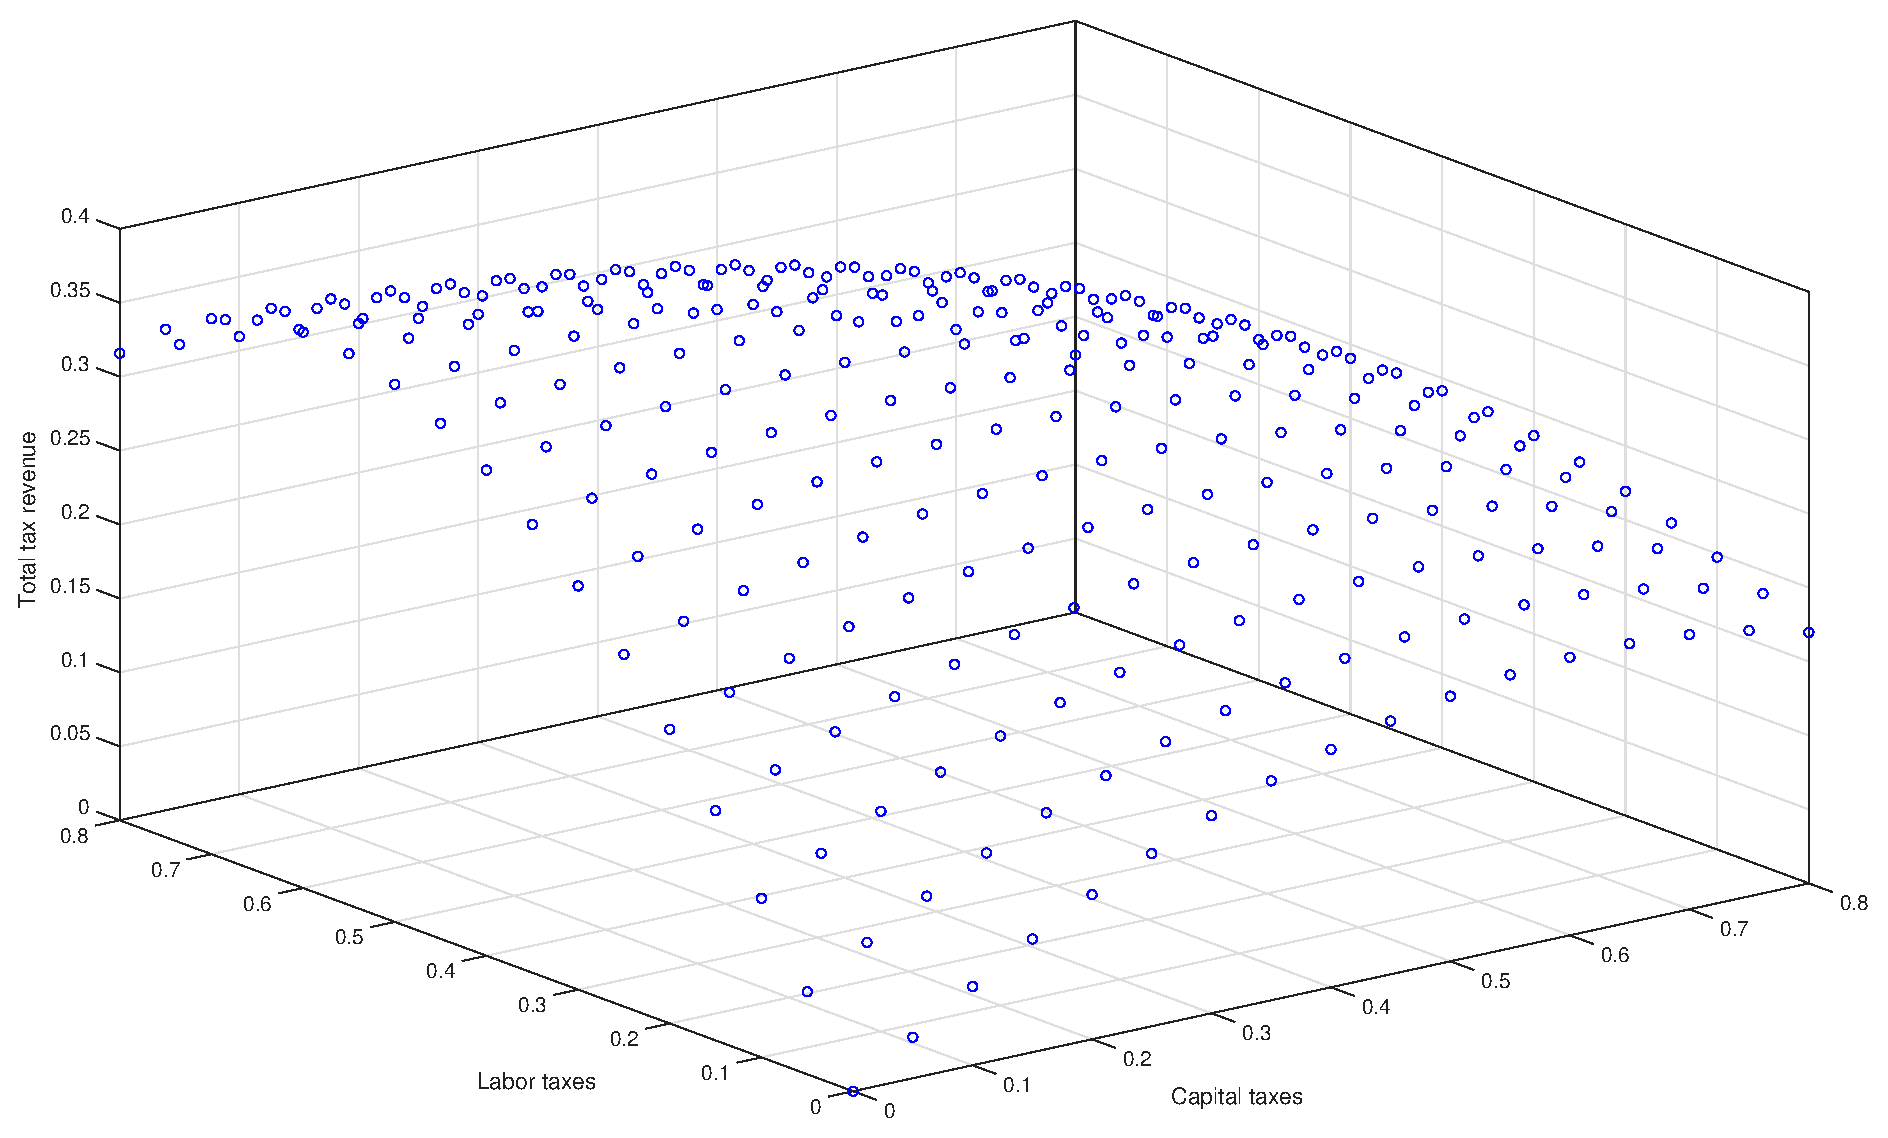
\includegraphics[width=\textwidth]{figures/total_tax_revenue.eps}%
    \end{figure}%
  \end{minipage}%
  \hfill%
  \begin{minipage}{0.48\textwidth}%
    \begin{small}%
      \begin{itemize}%
        \item[$\blacktriangleright$] Tax revenues are hump-shaped in either tax rate starting at 0.%
        \vspace*{0.15in}%
        \pause%
        \item[$\blacktriangleright$] In both tax rates, tax revenues are dome shaped, indicating an interior solution in maximizing revenues:%
        \begin{itemize}%
          \item[$\rightarrow$] Revenue-maximizing capital tax: $\tau_K^* \approx 0.05$ (revenue is almost flat for $\tau_K \leq 0.1$)%
          \item[$\rightarrow$] Revenue-maximizing labor tax: $\tau_L^* \approx 0.6$%
        \end{itemize}%
      \end{itemize}%
    \end{small}%
  \end{minipage}%
\end{frame}%
%-------------------------------------------------------------------------
% Quantitative Analysis: Interdependences of the Two Tax Rates
\begin{frame}{Quantitative Analysis: Interdependences of the Two Tax Rates}%
  \begin{minipage}{0.48\textwidth}%
    \begin{figure}
      \centering%
      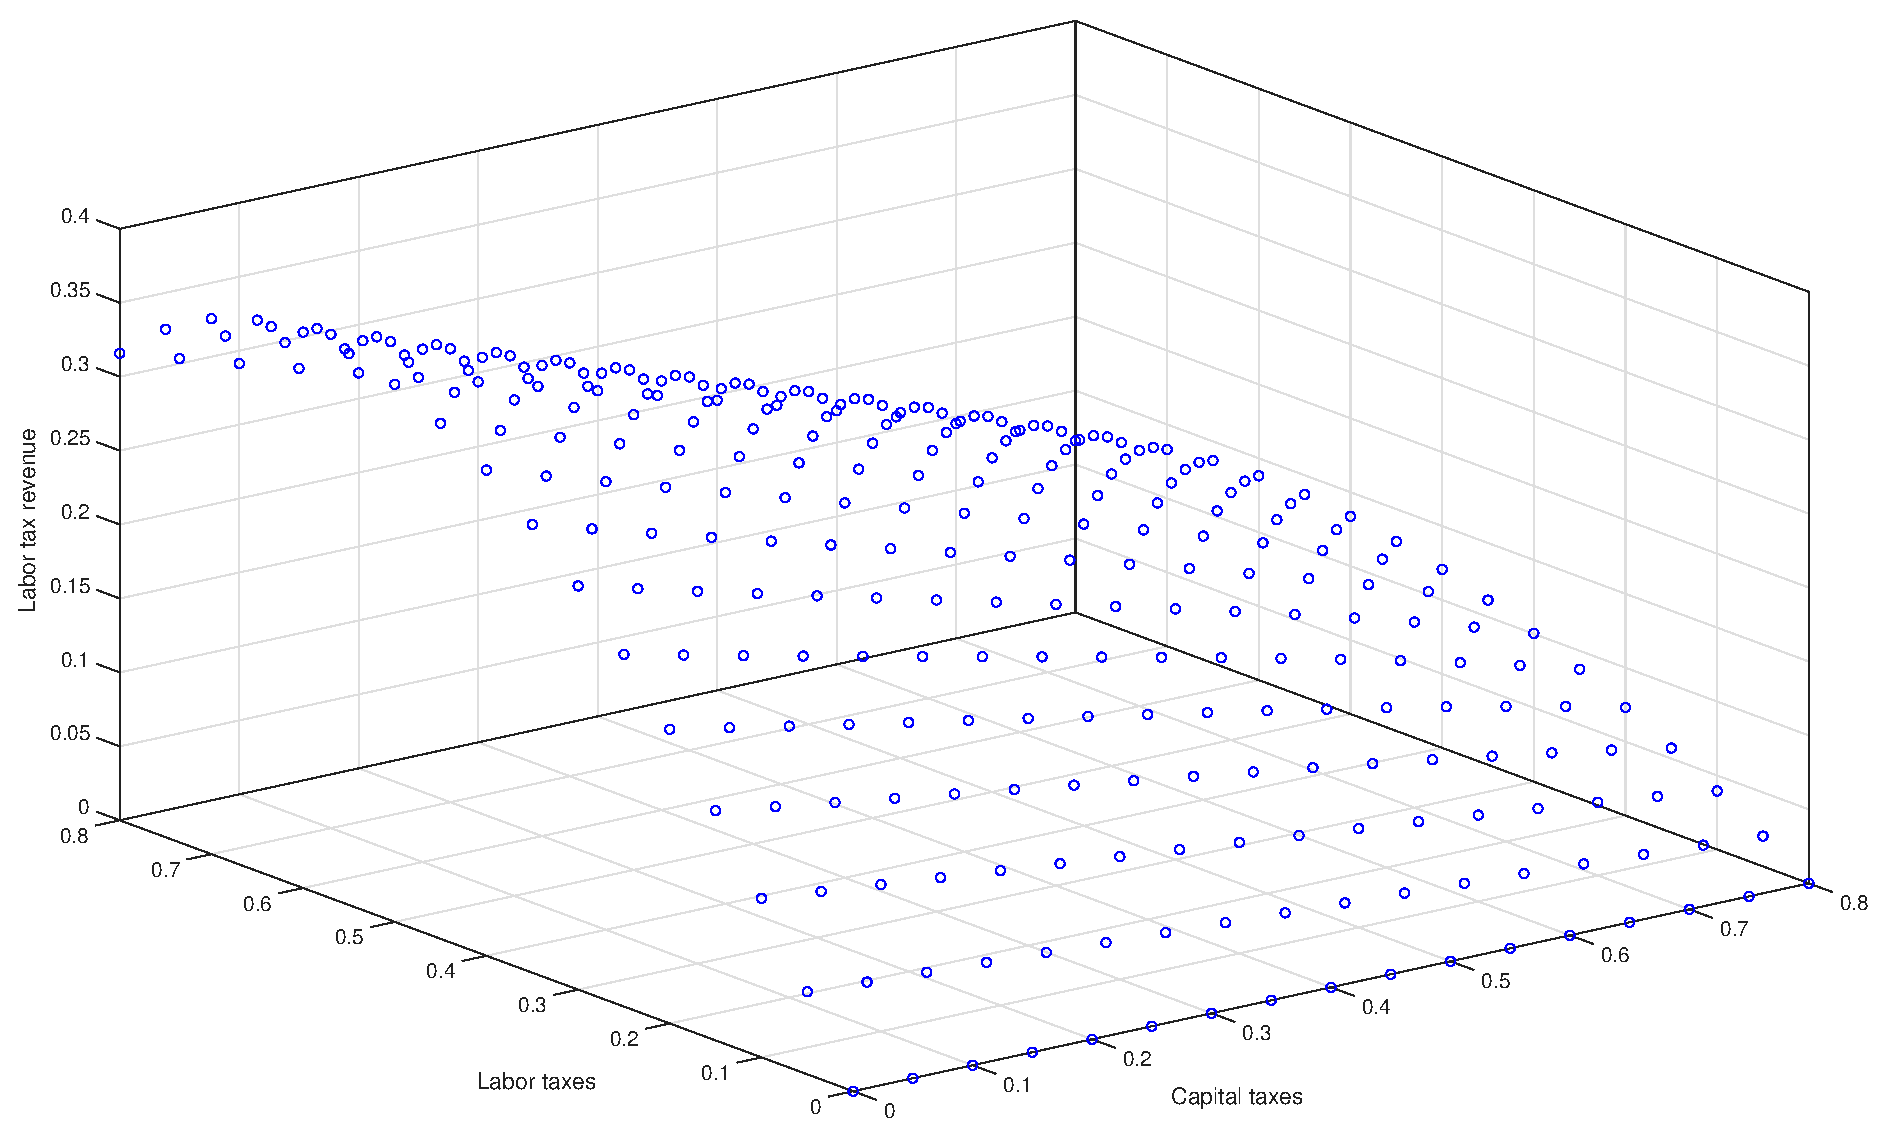
\includegraphics[width=0.75\textwidth]{figures/labor_tax_revenue.eps}\\%
      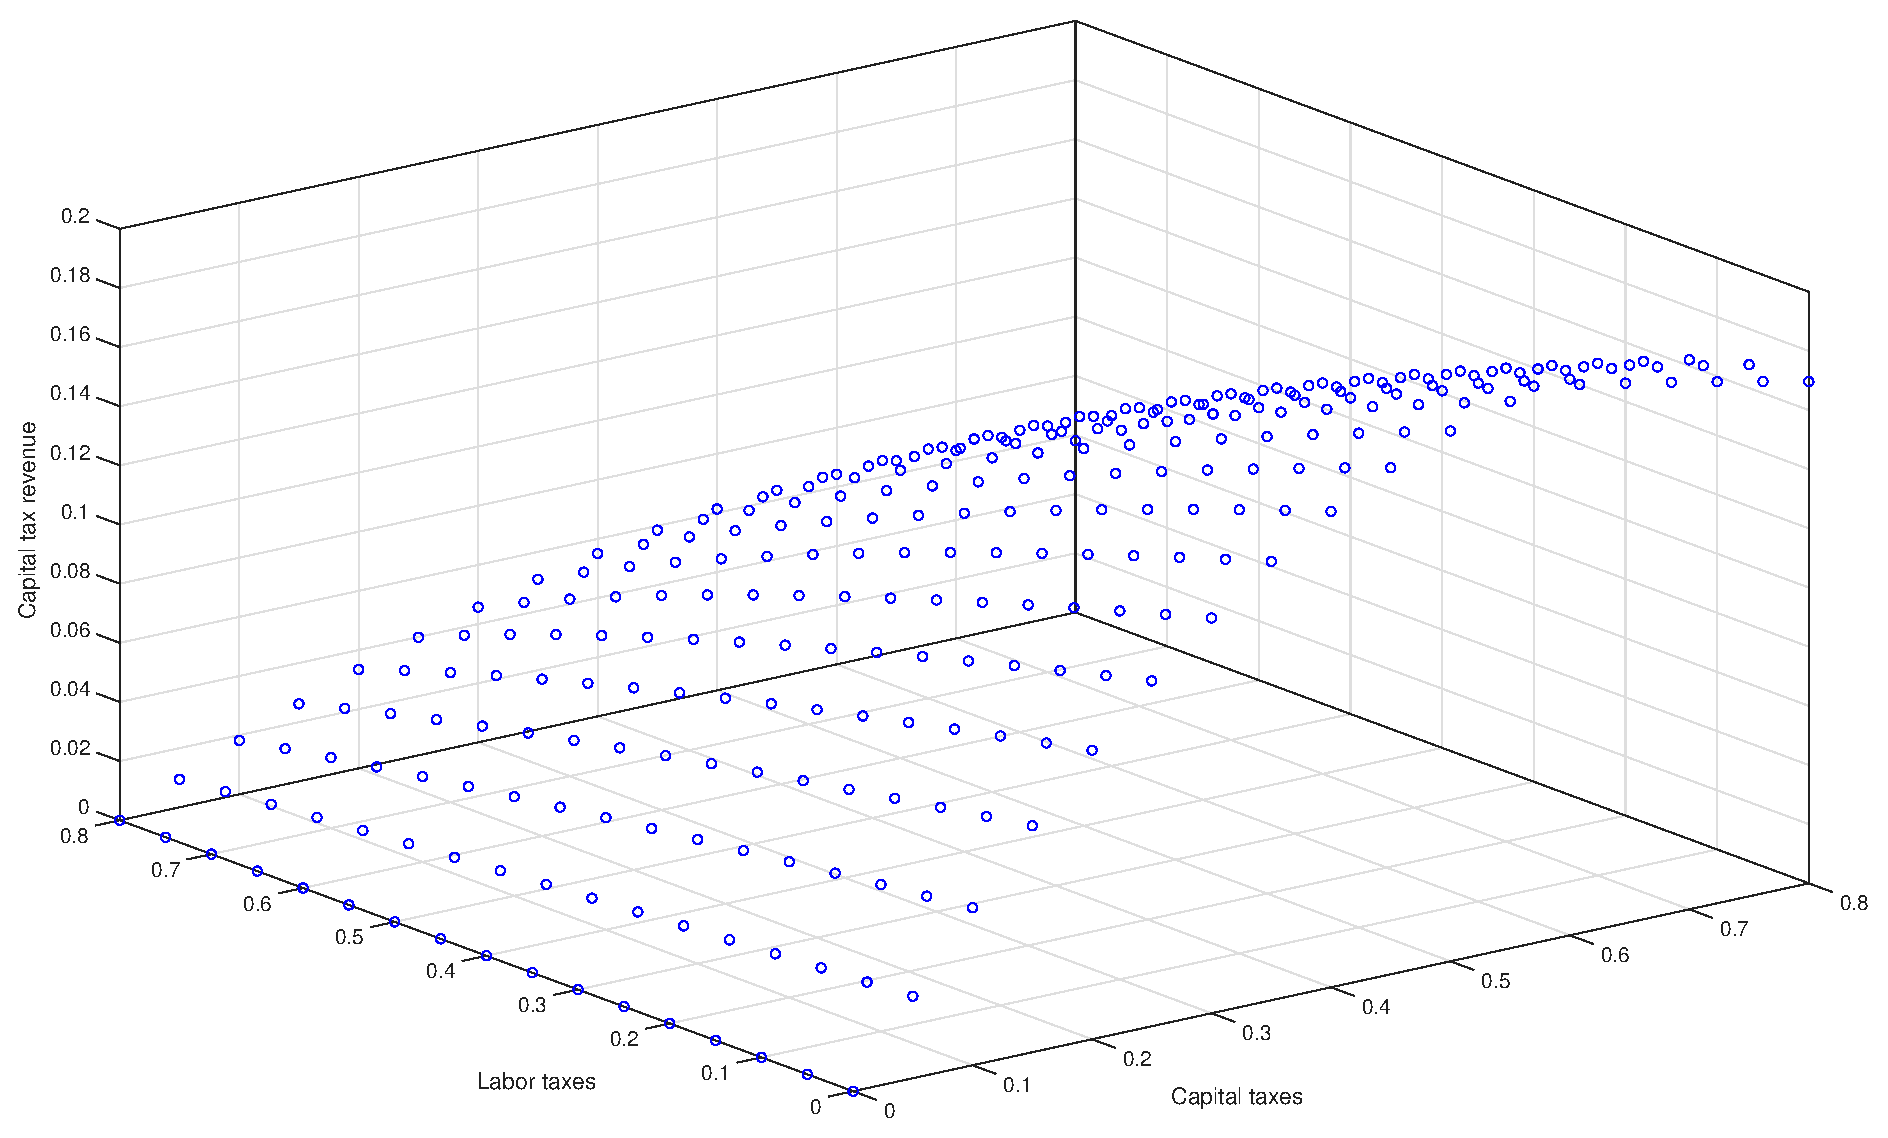
\includegraphics[width=0.75\textwidth]{figures/capital_tax_revenue.eps}%
    \end{figure}%
  \end{minipage}%
  \hfill%
  \begin{minipage}{0.5\textwidth}%
    \begin{small}%
      \begin{itemize}%
        \item[$\blacktriangleright$] Labor tax revenue is decreasing in the level of capital taxation and hump-shaped in labor taxation.%
        \vspace*{0.15in}%
        \pause%
        \item[$\blacktriangleright$] Increasing capital taxes steals a bit of revenue from labor taxation by discouraging capital accumulation!%
        \vspace*{0.15in}%
        \pause%
        \item[$\blacktriangleright$] The same pattern applies for capital taxation.%
      \end{itemize}%
    \end{small}%
  \end{minipage}%
\end{frame}%
%-------------------------------------------------------------------------
% Quantitative Analysis: Impact on Consumption and Labor
\begin{frame}{Quantitative Analysis: Impact on Consumption and Labor}%
  \begin{minipage}{0.48\textwidth}%
    \begin{figure}%
      \centering%
      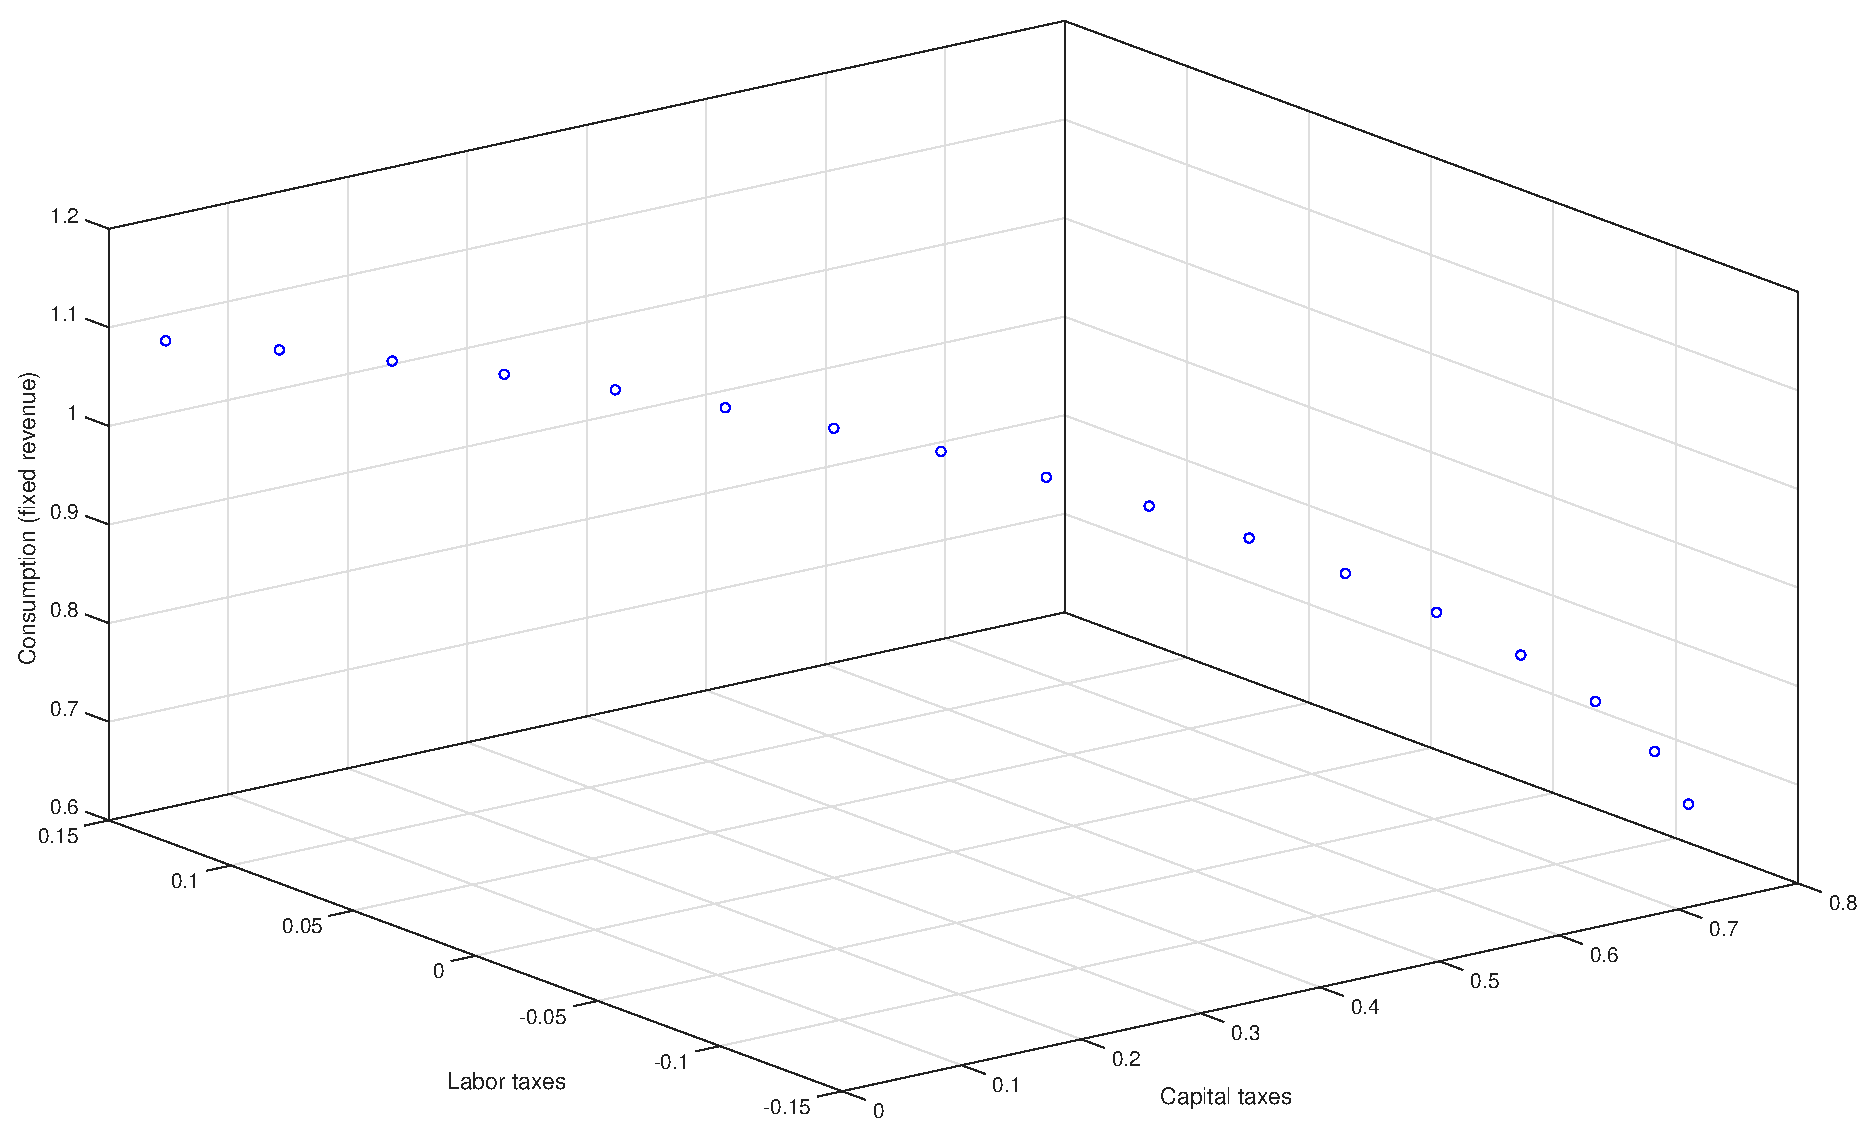
\includegraphics[width=0.75\textwidth]{figures/consumption_fixed_revenue.eps}\\%
      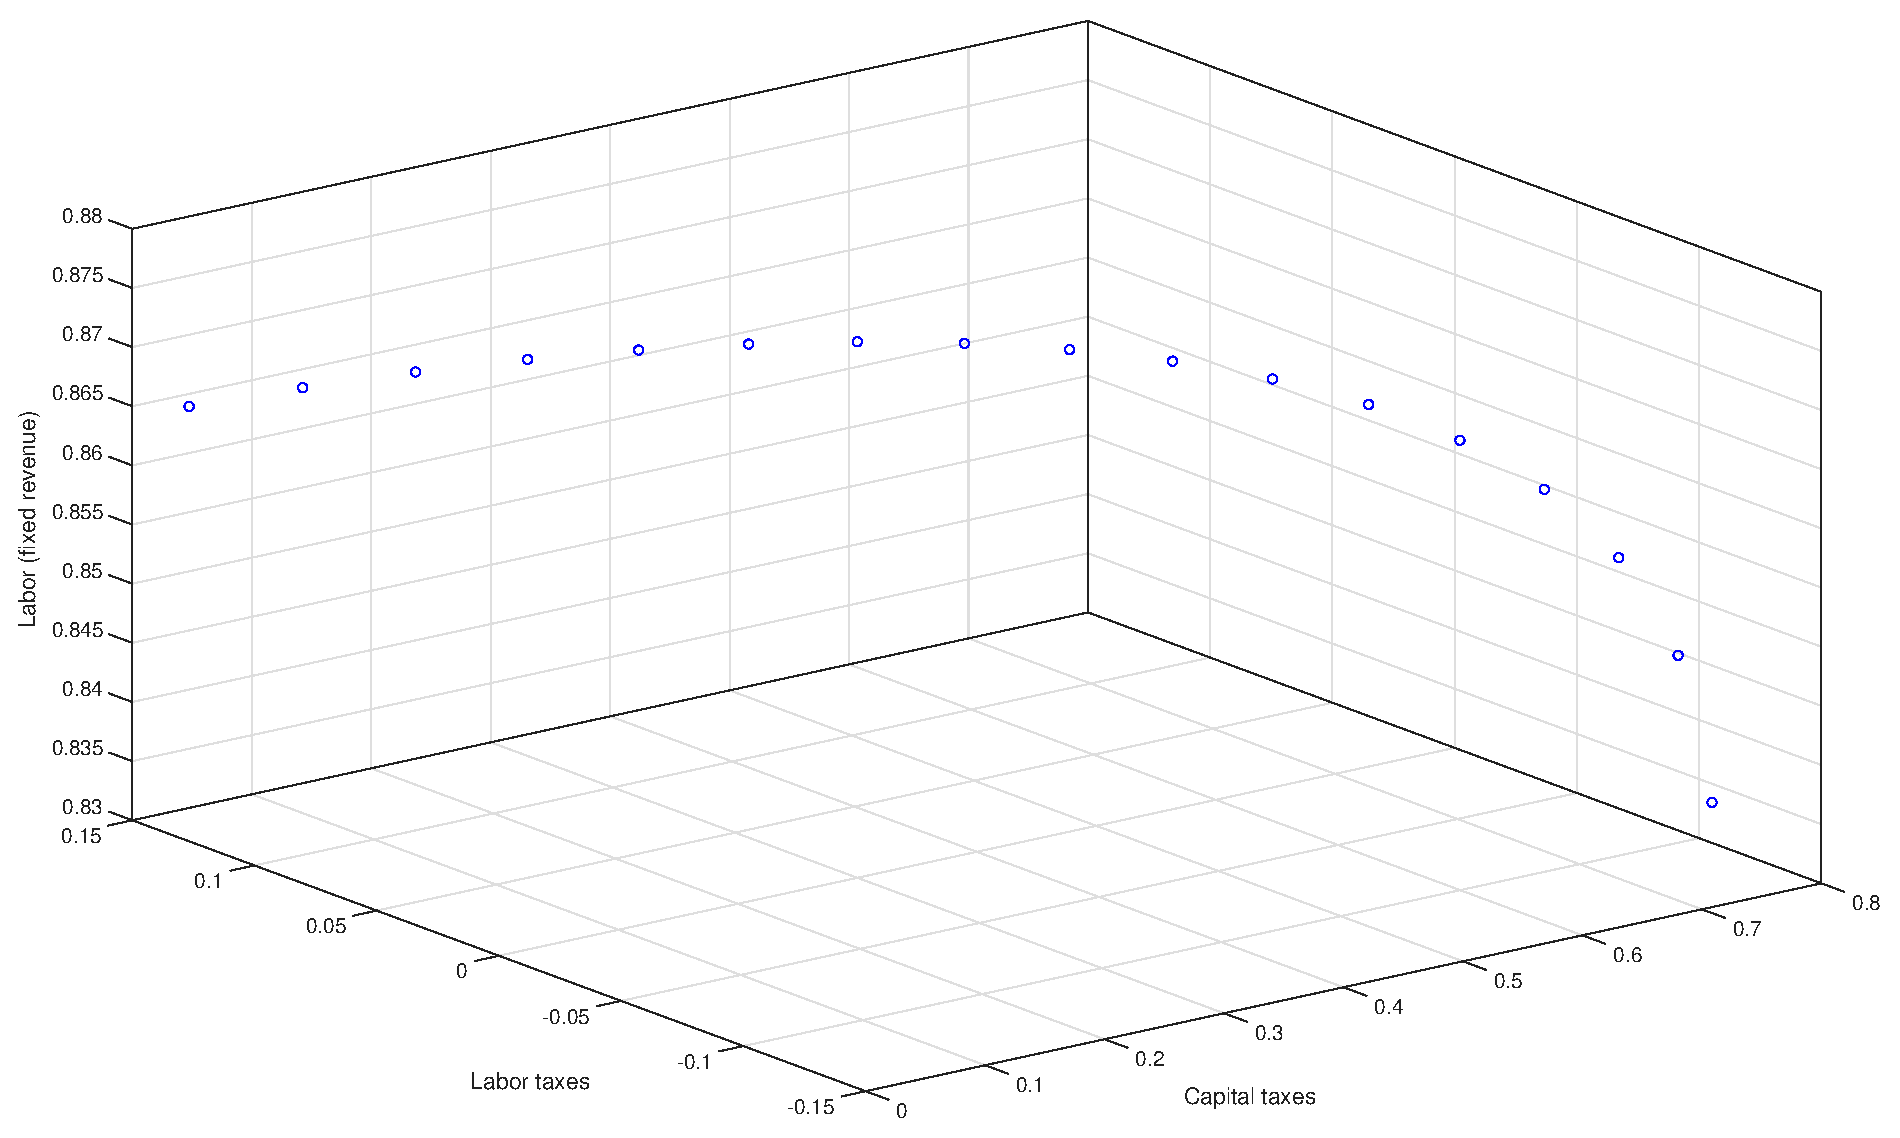
\includegraphics[width=0.75\textwidth]{figures/labor_fixed_revenue.eps}%
    \end{figure}%
  \end{minipage}%
  \hfill%
  \begin{minipage}{0.5\textwidth}%
    \begin{small}%
      \begin{itemize}%
        \item[$\blacktriangleright$] Fix tax revenue at: $\tau_K=0.3$ and $\tau_L=0$.%
        \item[$\blacktriangleright$] We calculate the impact on consumption and labor keeping overall tax revenue constant.%
        \vspace*{0.05in}%
        \pause%
        \item[$\blacktriangleright$] Consumption is decreasing in capital taxes!%
        \item[$\blacktriangleright$] Labor response is hump-shaped in capital taxes.%
        \item[$\blacktriangleright$] For $\tau_K > 0.3$, constant revenue requires a labor subsidy ($\tau_L < 0$).%
        \vspace*{0.05in}%
        \pause%
        \item[$\Rightarrow$] The model implies that \textbf{capital taxes are a bad way to raise tax revenue.}%
        \vspace*{0.05in}%
        \pause%
        \item[$\rightarrow$] How does this result depend on the model and its parameterization?%
        \item[$\rightarrow$] How does it depend on the impact of government spending on welfare?%
      \end{itemize}%
      \vspace*{-0.2in}%
    \end{small}%
  \end{minipage}%
\end{frame}%
%-------------------------------------------------------------------------
% Adding Government Expenditures
\begin{frame}{Adding Government Expenditures}%
  So far, we have assumed that any tax income is rebated lump-sum to the households. However, \textbf{government spending} can have many different positive benefits, for example:%
  \vspace*{0.1in}%
  \begin{itemize}%
    \item[$\blacktriangleright$] A direct utility benefit, e.g. public television or national defense.%
    \item[$\blacktriangleright$] A productive input, e.g. roads, bridges, and the legal system.%
    \item[$\blacktriangleright$] Insurance through various transfers.%
    \item[$\blacktriangleright$] Spending on education.%
    \item[$\blacktriangleright$] Spending on basic research, which affects productivity growth.%
  \end{itemize}%
  \vspace*{0.2in}%
  \pause%
  How does welfare and optimal taxes change once we introduce a non-wasteful government spending? \emph{See Cole (2020) chapter 18 for an analysis!}%
\end{frame}%
% %-------------------------------------------------------------------------
% % Simplifying the Tax System
% \begin{frame}{Simplifying the Tax System}%
%   We simplify the \textbf{government income side} ...%
%   \begin{itemize}%
%     \item[$\blacktriangleright$] Taxes are one-dimensional and are simply a flat rate output tax $\tau_Y$.%
%     \item[$\blacktriangleright$] There is no government debt, hence spending is equal to revenue (balanced budget).%
%   \end{itemize}%
%   \pause%
%   \vspace*{0.2in}%
%   Therefore, the \textbf{government budget constraint} is given by:%
%   \begin{align*}%
%     \omega G_{t+1} \; = \; \tau_Y Y_t%
%   \end{align*}%
%   \vspace*{-0.3in}%
%   \begin{itemize}%
%     \item[$\blacktriangleright$] $\omega>1$ is our model of government waste or inefficiency.%
%     \item[$\blacktriangleright$] \emph{Government CiA constraint:} Revenue that is collected today funds expenditure in the next period.%
%   \end{itemize}%
% \end{frame}%
% %-------------------------------------------------------------------------
% % Utility and Production with Government Spending
% \begin{frame}{Utility and Production with Government Spending}%
%   We assume that government spending is divided into ...%
%   \vspace*{0.1in}%
%   \begin{itemize}%
%     \item[$\blacktriangleright$] a fraction $\psi$ of spending that works as a consumption good. It leads to a \textbf{modified household utility function:}%
%     \begin{align*}%
%       u(C) - v(L) + h(\psi G)%
%     \end{align*}%
%     \pause%
%     \item[$\blacktriangleright$] a fraction $1-\psi$ that works as a production input. It leads to a \textbf{modified production function:}%
%     \begin{align*}%
%       Y \; = \; f(ZL,K,(1-\psi)G)%
%     \end{align*}%
%   \end{itemize}%
% \end{frame}%
% %-------------------------------------------------------------------------
% % Functional Forms of Government Spending
% \begin{frame}{Functional Forms of Government Spending}%
%   What are appropriate functional forms for $h(\cdot)$ and $f(\cdot)$? We want something that is rationalized by the data!%
%   \vspace*{0.1in}%
%   \pause%
%   \begin{itemize}%
%     \item[$\blacktriangleright$] \textbf{Preferences:} Unless we want consumption and government spending crowding out each other, the functional forms should be the same. This suggests:%
%     \begin{align}%
%       u(\cdot) \; = \; a \times h(\cdot)%
%     \end{align}%
%     \vspace*{0.1in}%
%     \pause%
%     \item[$\blacktriangleright$] \textbf{Production:} It is common to use a constant-elasticity-of-substitution (CES) production function as it matches the data well. Here, we use its special case of a Cobb-Douglas function:%
%     \begin{align}%
%       Y \; = \; (ZL)^{1-\alpha-\nu} K^{\alpha} ((1-\psi)G)^{\nu} \label{eq:EndoG_Prod2}%
%     \end{align}%
%   \end{itemize}%
% \end{frame}%
% %-------------------------------------------------------------------------
% % Household Optimization with Government Spending
% \begin{frame}{Household Optimization with Government Spending}%
%   \begin{block}{Return to the basic model}%
%     Since there is just an output tax, we can back to our basic model with HH production and no rental market for labor and capital.%
%   \end{block}%
%   The household maximizes her utility following:%
%   \begin{align*}%
%     \max_{\left\{ C_{t},L_{t},M_{t},B_{t+1},K_{t+1}\right\}_{t=1}^{2}} \sum_{t=1,2}\beta^{t-1}\left[ u(C_{t})-v(L_{t}) + h(\psi G_t) \right] +\beta^{2} V(M_{3},B_{3},K_{3})%
%   \end{align*}%
%   \pause%
%   subject to%
%   \begin{align*}%
%     M_{t} \; \geq \; P_{t} C_{t}%
%   \end{align*}%
%   and%
%   \begin{align*}%
%     & P_{t}\left[ (1-\tau_Y) \left[ Z_{t} L_{t} \right]^{1-\alpha-\nu} K_{t}^{\alpha}((1-\psi) G_t)^{\nu} - \delta K_{t} \right] + \left[ M_{t}-P_{t}C_{t} \right] + B_{t} + T_{t} \\%
%     \geq \; & M_{t+1} + q_{t} B_{t+1} + P_{t} \left[ K_{t+1}-K_{t} \right] \quad \forall t\leq 2%
%   \end{align*}%
%   \pause%
%   \vspace*{-0.15in}%
%   \begin{small}%
%     \begin{itemize}%
%       \item[$\Rightarrow$] The FOCs are \textbf{largely unchanged}, but we do need to take account of the tax on output.%
%     \end{itemize}%
%   \end{small}%
% \end{frame}%
% %-------------------------------------------------------------------------
% % Household FOCs with Government Spending
% \begin{frame}{Household FOCs with Government Spending}%
%   \begin{small}%
%     \text{Consumption condition:}%
%     \begin{align}%
%       \beta^{t-1} u^{\prime}(C_{t}) - P_{t} \left[ \lambda_{t}+\mu_{t} \right] \; \overset{!}{=} \; 0%
%     \end{align}%
%     \pause%
%     \text{Labor condition:}%
%     \begin{align}%
%       -\beta^{t-1} v^{\prime}(L_{t}) + \mu_{t} P_{t} \alert{(1-\tau_Y)} Z_{t}^{1-\alpha-\nu} (1-\alpha-\nu) L_{t}^{-\alpha-\nu} K_{t}^{\alpha} \alert{((1-\psi) G_t)^{\nu}} \; \overset{!}{=} \; 0%
%     \end{align}%
%     \pause%
%     \text{Capital condition:}%
%     \begin{align}%
%       -\mu_{t} P_{t} + \mu_{t+1} P_{t+1} \left[ \alert{(1-\tau_Y)} \left[ Z_{t+1} L_{t+1} \right]^{1-\alpha-\nu} \alert{((1-\psi)G_t)^{\nu}} \alpha K_{t+1}^{\alpha-1} + 1 - \delta \right] \; \overset{!}{=} \; 0%
%     \end{align}%
%     \pause%
%     \text{Money condition:}%
%     \begin{align}%
%       -\mu_{t} + \lambda_{t+1} + \mu_{t+1} \; \overset{!}{=} \; 0%
%     \end{align}%
%     \pause%
%     \text{Bonds condition:}%
%     \begin{align}%
%       -\mu_{t} q_{t} + \mu_{t+1} \; \overset{!}{=} \; 0%
%     \end{align}%
%   \end{small}%
%   \vspace*{-0.2in}%
% \end{frame}%
% %-------------------------------------------------------------------------
% % Solving for the Balanced-Growth-Path (1/2)
% \begin{frame}{Solving for the Balanced-Growth-Path (1/2)}%
%   \textbf{Assume:} 1) Perfect foresight, 2) constant growth rates, 3) government spending grows at rate of productivity. We can collect our usual expressions of the balanced growth path and get the following set of equations:%
%   \pause%
%   \begin{small}%
%     \begin{enumerate}%
%       \item \textbf{Government spending condition} (deflated by $1+g$ due to gov. CiA constraint):%
%       \begin{align}%
%         G_{1}^{1-\nu} \; = \; \frac{1}{1+g}\frac{\tau_Y}{\omega} L^{1-\alpha-\nu} K_1^{\alpha} (1-\psi)^{\nu} \label{eq:EndoG_G}%
%       \end{align}%
%       \vspace*{-0.1in}%
%       \pause%
%       \item \textbf{Resource constraint:}%
%       \begin{align}%
%         C_1 \; = \; (1-\tau_Y) L^{1-\alpha-\nu} K_1^{\alpha} ((1-\psi)G_1)^{\nu} - \left[ g+\delta \right] K_{1} \label{eq:EndoG_C}%
%       \end{align}%
%       \vspace*{-0.1in}%
%       \pause%
%       \item \textbf{Labor condition:}%
%       \begin{align}%
%         L^{\gamma+\alpha+\nu} \; = \; \frac{\beta}{1+\tau}\frac{(1-\tau_Y)}{C_1}(1-\alpha-\nu) K_{1}^{\alpha} ((1-\psi)G_1)^{\nu} \label{eq:EndoG_L}%
%       \end{align}%
%       \vspace*{-0.1in}%
%       \pause%
%       \item \textbf{Capital condition:}%
%       \begin{align}%
%         1 \; = \; \frac{\beta}{1+g} \left\{ (1-\tau_Y) \alpha L^{1-\alpha-\nu} K_1^{\alpha-1} ((1-\psi)G_1)^{\nu} +1-\delta \right\} \label{eq:EndoG_K}%
%       \end{align}%
%     \end{enumerate}%
%   \end{small}%
% \end{frame}%
% %-------------------------------------------------------------------------
% % Solving for the Balanced-Growth-Path (2/2)
% \begin{frame}{Solving for the Balanced-Growth-Path (2/2)}%
%   \begin{small}%
%     \begin{enumerate}%
%       \item Start with (\ref{eq:EndoG_G}) and rearrange for $\frac{G_1}{L}$ and $\frac{K_1}{L}$ to get:%
%       \begin{align}%
%         \left[ \frac{G_{1}}{L} \right]^{1-\nu} \; = \; \frac{1}{1+g} \frac{\tau_Y}{\omega} \left[ \frac{K_1}{L} \right]^{\alpha} (1-\psi)^{\nu}\label{eq:GoverL}% 
%       \end{align}%
%       \pause%
%       \item Rearrange (\ref{eq:EndoG_K}) for $\frac{K_1}{L}$ to get:%
%       \begin{align}%
%         1 \; = \; \frac{\beta }{1+g} \left\{ (1-\tau_Y) \alpha \left[ \frac{K_1}{L} \right]^{\alpha-1} \left( (1-\psi)\left[ \frac{G_{1}}{L} \right] \right)^{\nu} +1-\delta \right\} \label{eq:KoverL}%
%       \end{align}%
%       \pause%
%       \item Plug (\ref{eq:GoverL}) into (\ref{eq:KoverL}) to get:%
%       \begin{align}%
%         1 \; = \;  \frac{\beta}{1+g} \left\{ (1-\tau_Y) \alpha \left[ \frac{K_1}{L} \right]^{\alpha-1} (1-\psi)^{\nu}  \left[ \frac{1}{1+g} \frac{\tau_Y}{\omega}  \left[ \frac{K_1}{L} \right]^{\alpha} (1-\psi)^{\nu} \right]^{\frac{\nu}{1-\nu}} +1-\delta \right\}%
%       \end{align}%
%       \pause%
%       \item Lastly, use the above results and solve for (\ref{eq:EndoG_L}) to get:%
%       \begin{align}%
%         L^{1+\gamma} \; = \; \frac{\beta}{1+\tau} \frac{(1-\tau_Y)}{C_1} (1-\alpha-\nu) Y_1%
%       \end{align}%
%     \end{enumerate}%
%   \end{small}%
% \end{frame}%
%-------------------------------------------------------------------------
% REFERENCES AND APPENDIX
%-------------------------------------------------------------------------
\section{Conclusion}%
%-------------------------------------------------------------------------
% Summarizing the Lecture
\begin{frame}{Summarizing the Lecture}%
  \begin{center}%
    \begin{large}%
      Can you summarize the three main aspects of the lecture?%
    \end{large}%
  \end{center}%
\end{frame}%
%-------------------------------------------------------------------------
% Concluding Remarks
\begin{frame}{Concluding Remarks}%
  \begin{block}{Big Picture of the Lecture:}%
    \begin{enumerate}%
      \item How does capital change the behavior of our model economy?%
      \item How do taxes and government spending impact our model economy?%
      \item Can we derive some policy prescriptions from the model?%
    \end{enumerate}%
  \end{block}%
  \pause%
  \begin{itemize}%
    \item[$\blacktriangleright$] Capital is a \textbf{productive input factor} and accumulates along productivity increases!%
    \begin{itemize}%
      \item[$\rightarrow$] Labor productivity depends on the capital stock.%
      \item[$\rightarrow$] Kaldor facts are replicated by the model framework.%
    \end{itemize}%
    \vspace*{0.1in}%
    \pause%
    \item[$\blacktriangleright$] Both capital and labor \textbf{taxes have a distortionary impact} on the allocation of their respective input factor!%
    \begin{itemize}%
      \item[$\rightarrow$] Capital taxes reduce the capital-to-labor ratio in the economy.%
      \item[$\rightarrow$] Labor taxes reduce the level of labor supply in the economy.%
    \end{itemize}%
    \vspace*{0.1in}%
    \pause%
    \item[$\blacktriangleright$] A combination of capital and labor taxes raises the \textbf{highest tax revenue!}%
    \begin{itemize}%
      \item[$\rightarrow$] However, capital taxes monotonically reduce consumption.%
      \item[$\rightarrow$] We have to include non-wasteful government spending in the analysis to give a more in-depth analysis of optimal fiscal policy.%
    \end{itemize}%
  \end{itemize}%
  \vspace*{-0.1in}%
\end{frame}%
%-------------------------------------------------------------------------
% References
\begin{frame}{References}%
  \begin{footnotesize}%
    \begin{itemize}%
      \item[$\blacktriangleright$] Kaldor, N. (1961). Capital accumulation and economic growth. In The Theory of capital: proceedings of a conference held by the International Economic Association (pp. 177-222). London: Palgrave Macmillan UK.%
      \item[$\blacktriangleright$] Harold L. Cole (2020). Monetary and Fiscal Policy through a DSGE Lens. Oxford University Press.%
    \end{itemize}%
  \end{footnotesize}%
\end{frame}%
%-------------------------------------------------------------------------
\end{document}%